\section{Performance Modeling: Parameter Identification (5/5 Points)}

\subsection{Task 1a - PCI Express latency for \texttt{cudaMemcpy()} in $\mu \mathrm{s}$ (1 Point)}
In order to find the latencies for the \texttt{K40 Tesla} and the \texttt{RTX 3060} GPU's, the assumption is made that timings
one is able to measure with \texttt{timer.hpp} and \texttt{<iostream>} the following quantities: a latency $\ell$, a constant time for \texttt{cudaMemcpy()}'ing one
\texttt{double} called $T_{\texttt{double}}$, two timings one measures $T_1$ and $T_2$ and an arbitrary positive integer N to \texttt{cudaMemcpy()} a vector of doubles
of length N.

\begin{align*}
  \ell + &T_{\texttt{double}} = T_1 \\
  \ell +  &\mathrm{N} \cdot T_{\texttt{double}} = T_2 \\
\rightarrow \ell &= \frac{T_2 - T_1 \cdot \mathrm{N}}{1 - \mathrm{N}} 
\end{align*}

With this model assumption one can obtain the latency  $\ell$ for both devices. The calculation of the above equation can be seen in the listing below in
line 28.

\begin{lstlisting}[language=C++, title=C++ Cuda Code Obtaining the latency]
int N = 1e7;
double *x = (double *)malloc(sizeof(double));
double *x_N = (double *)malloc(sizeof(double) * N);
*x = 1;
std::fill(x_N, x_N + N, 1);
double *cuda_x, *cuda_x_N;
cudaMalloc(&cuda_x, sizeof(double));
cudaMalloc(&cuda_x_N, sizeof(double) * N);

std::vector<double> timings_double(100, 0.0);
std::vector<double> timings_N_doubles(100, 0.0);

for (size_t i=0; i<=100; ++i){
  timer.reset();
  cudaMemcpy(cuda_x, x, sizeof(double), cudaMemcpyHostToDevice);
  cudaDeviceSynchronize();
  timings_double[i] = timer.get();
}
double timing_double = findMedian(timings_double, 100);

for (size_t i=0; i<=100; ++i){
  timer.reset();
  cudaMemcpy(cuda_x_N, x_N, sizeof(double)*N, cudaMemcpyHostToDevice);
  timings_N_doubles[i] = timer.get();
  cudaDeviceSynchronize();
}
double timing_N_doubles = findMedian(timings_N_doubles, 100);
double latency = (timing_N_doubles - timing_double*N)/(1-N);
\end{lstlisting}

\texttt{PCI Express gen3 Latency on RTX3060: 3.99926 $\mu$s} \newline
\texttt{PCI Express gen3 Latency on K40 TESLA: 8.9987 $\mu$s}

\pagebreak


\subsection{Task 1b - Kernel Launch Latency in $\mu \mathrm{s}$ (1 Point)}
Task 1b is relatively straight forward, just launch a high number of empty kernels with \texttt{<<<1,1>>>} and find the median time!

\begin{lstlisting}[language=C++, title=C++ Cuda Code for Kernel Launch Latency]
__global__ void cuda_5_1b()
{
// Kennt's ihr eh Spiegeldondi? - Mahatma Ghandi, ca. 1940 - idea of an empty Kernel..
}
int main() {

Timer timer;
std::vector<double> timings(100, 0.0);

for (size_t i=0; i<100; ++i){
  timer.reset();
  cuda_5_1b<<<1, 1>>>();
  cudaDeviceSynchronize();
  timings[i] = timer.get();
  cudaDeviceSynchronize();
}
double latency = findMedian(timings, 100);
std::cout << "Kernel Launch Latency: " << latency << std::endl;
\end{lstlisting}

\texttt{Kernel Launch Latency on RTX3060: 10 $\mu$s} \newline
\texttt{Kernel Launch Latency on K40 TESLA: 5 $\mu$s}



\pagebreak


\subsection{Task 1c - Practical Peak Memory Bandwidth in GB/s (1 Point)}
The Numbers for the obtained Peak Memory Bandwidth are in the legend of Figure \ref{label_1c_figure} and the relevant code chunks in the listing below.

\begin{lstlisting}[language=C++, title=C++ Cuda Code for Peak Memory Bandwidth]
__global__ void cuda_5_1c(double *x, double *y, double *z, int N)
{
  unsigned int total_threads = blockDim.x * gridDim.x;
	unsigned int global_tid = blockIdx.x * blockDim.x + threadIdx.x;
  for (unsigned int i = global_tid; i<N; i += total_threads) {
		z[i] = x[i] + y[i];
	}

}

for(int j=0; j < median_int; j++){
  cudaDeviceSynchronize();
  timer.reset();
  cuda_5_1c<<<((N_vec[i]+255)/256), 256>>>(gpu_x, gpu_y, gpu_z, N_vec[i]);
  cudaDeviceSynchronize();
  timings.push_back(timer.get());
}

peak_bw.push_back((3*N_vec[i]*sizeof(double)*pow(10,-9))/findMedian(timings, median_int));
timings.clear();
std::cout << N_vec[i] << ", " << peak_bw[i] << std::endl;
\end{lstlisting}

\begin{figure}[h]
  \begin{center}
    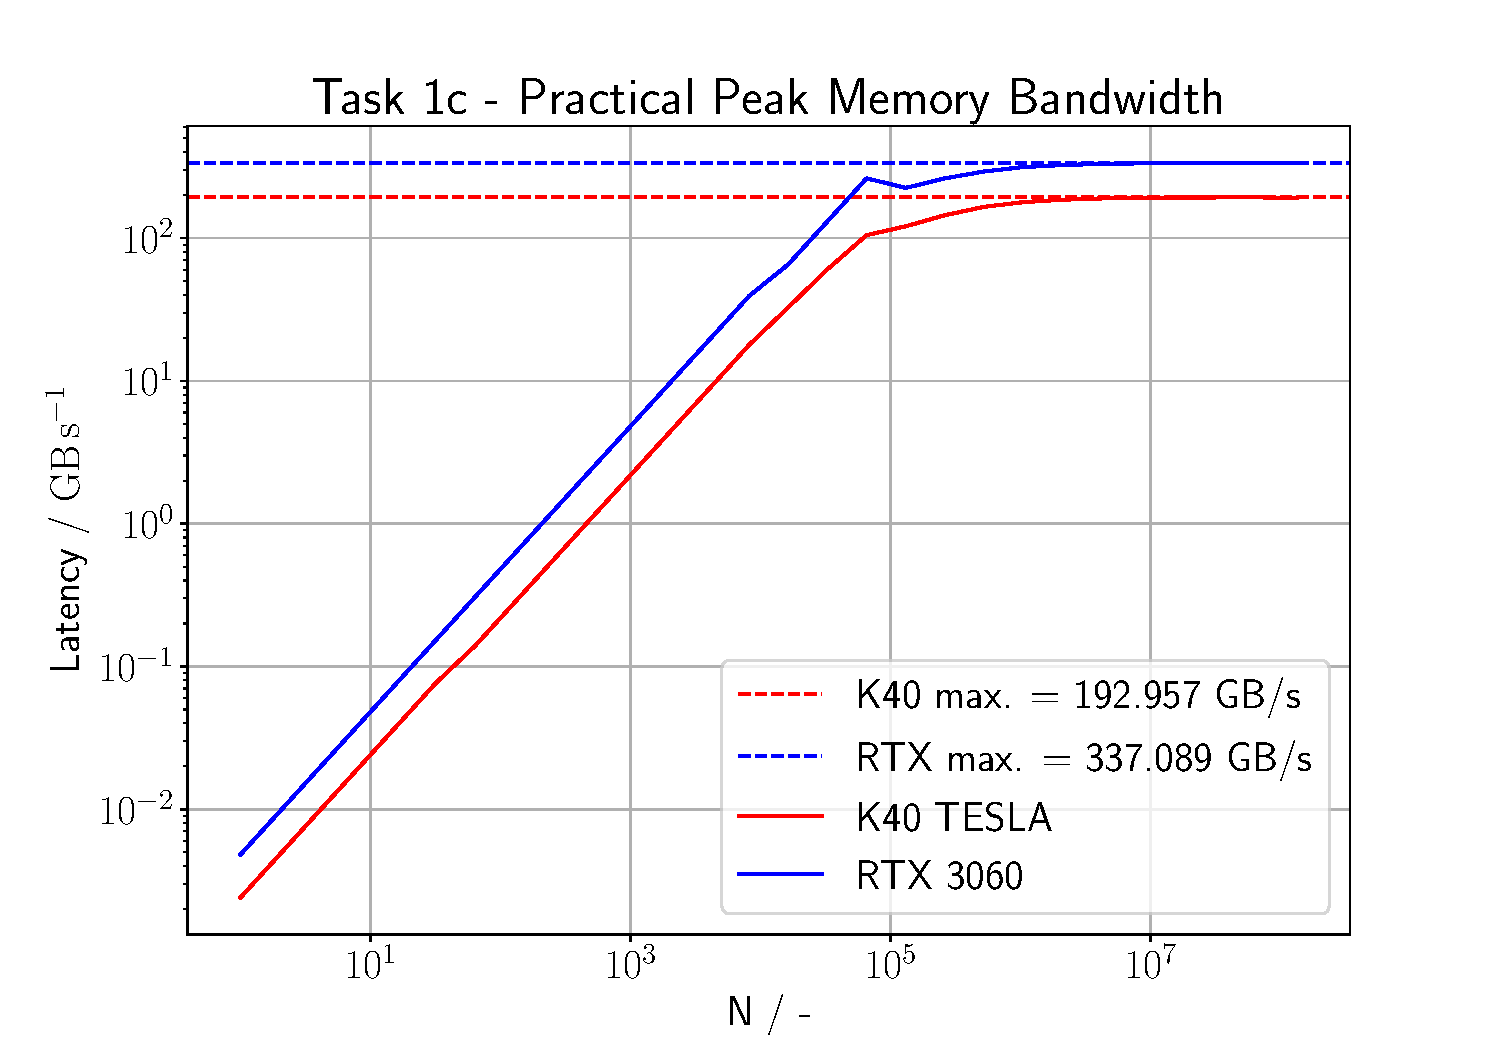
\includegraphics[width= 0.8\linewidth]{figures/task_1_c.pdf}
    \caption{Results for Task 1c}
    \label{label_1c_figure}
  \end{center}
\end{figure}



\pagebreak

\subsection{Task 1d - Maximum Number of \texttt{atomicAdd()} / s}
The Numbers for the obtained \texttt{atomicAdd()}'s per second are in the legend of Figure \ref{label_1d_figure} and the relevant code chunks in the listing below.

\begin{lstlisting}[language=C++, title=C++ Cuda Code for Maximum number of \texttt{atomicAdd()}]
__global__ void cuda_5_1d(double *atomic_add_result)
{
	atomicAdd(atomic_add_result, threadIdx.x);
}
   
    for (size_t i=0; i<N_max; ++i){

        for(int j=0; j < median_int; j++){
            cudaDeviceSynchronize();
            timer.reset();
            cuda_5_1d<<<(int)N_vec[i], 1>>>(x_gpu);
            cudaDeviceSynchronize();
            timings.push_back(timer.get());
        }

    median_timings.push_back(findMedian(timings, median_int));
    timings.clear();
    std::cout << N_vec[i] << ", " << N_vec[i]/median_timings[i] << std::endl;
    }

    return EXIT_SUCCESS;
}


\end{lstlisting}

\begin{figure}[h]
  \begin{center}
    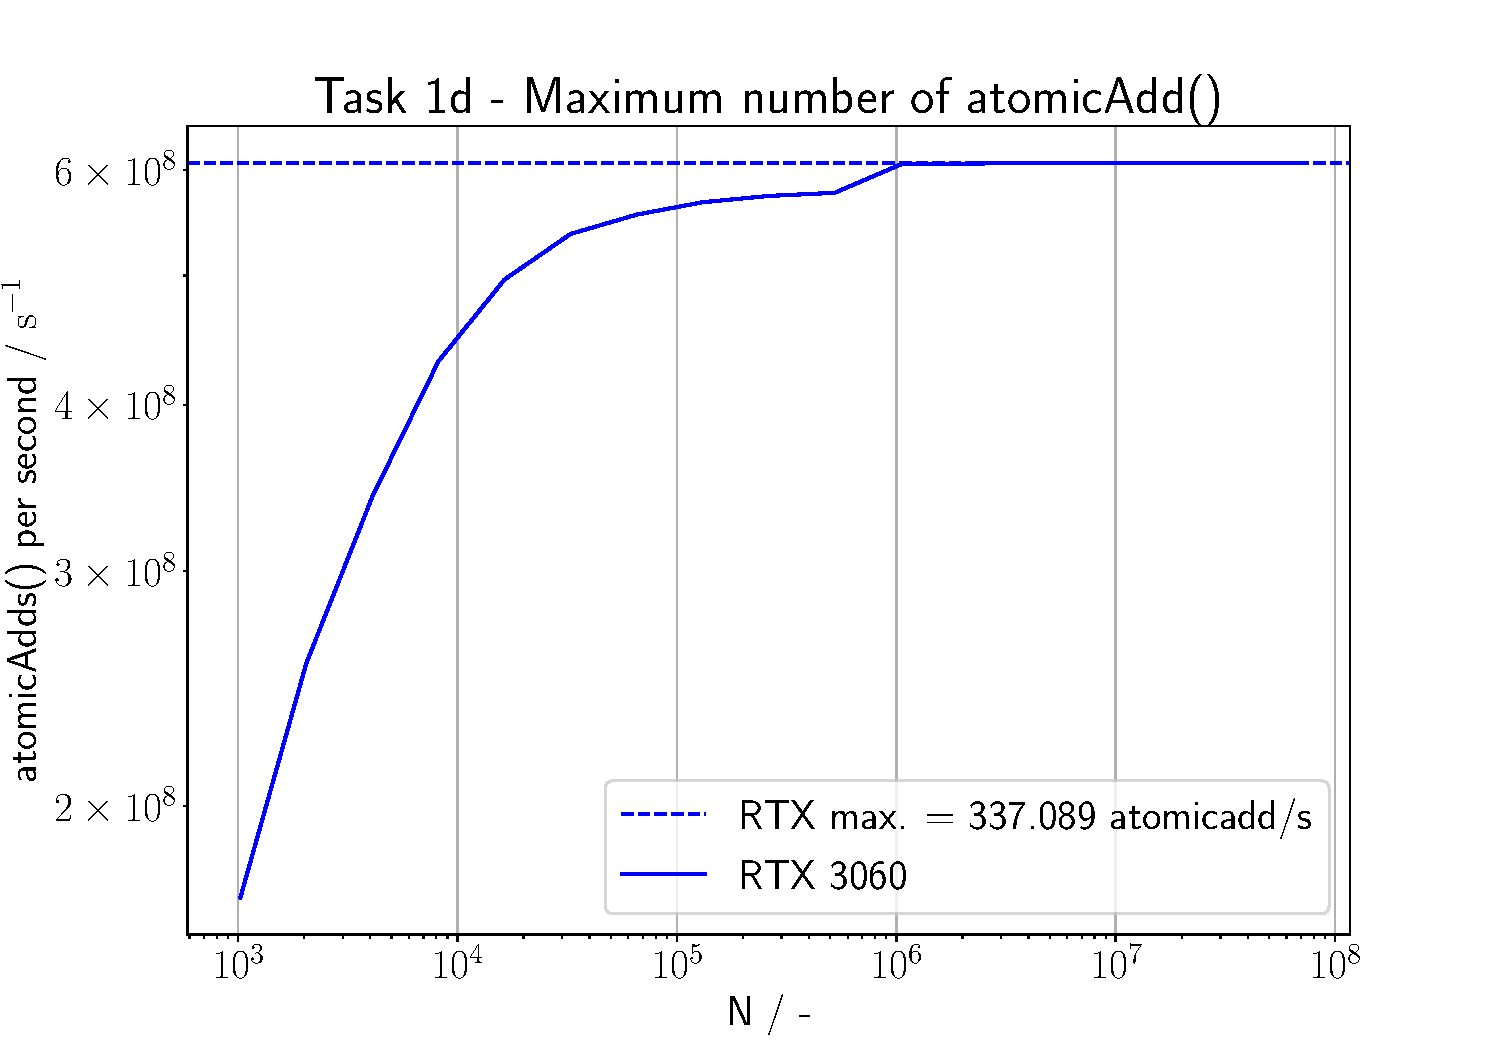
\includegraphics[width= 0.8\linewidth]{figures/task_1_d.pdf}
    \caption{Results for Task 1d}
    \label{label_1d_figure}
  \end{center}
\end{figure}



\pagebreak

\subsection{Task 1e - Peak FLOP's (i.e. $\alpha += \beta \cdot \gamma$) for \texttt{double}'s as GFLOPs/s (1 Point)}
The Numbers obtained for the Peak Floating Point Rate for both GPU's are in the legend of figure \ref{label_1e_figure} and the relevant
code chunks in the listing below.

\begin{lstlisting}[language=C++, title=C++ Cuda Code Maximal Floating Point Rate]
__global__ void cuda_5_1c(double *x, double *y, double *z, int N)
{
  float a = x[blockIdx.x*blockDim.x + threadIdx.x];
  float b = y[blockIdx.x*blockDim.x + threadIdx.x];
  float c;
  for (int i = 0; i < 8*3000; i++) {
    c += a * b;
  }
  z[blockIdx.x*blockDim.x + threadIdx.x] += c;
}

for (size_t i=0; i<N_max-N_min; ++i){
  for(int j=0; j < median_int; j++){
    cudaDeviceSynchronize();
    timer.reset();
    cuda_5_1c<<<((N_vec[i]+255)/256), 256>>>(gpu_x, gpu_y, gpu_z, N_vec[i]);
    cudaDeviceSynchronize();
    timings.push_back(timer.get());
  }
  peak_flops.push_back((2*8*3000*N_vec[i]* pow(10, -9))/findMedian(timings, median_int));
  timings.clear();
  std::cout << N_vec[i] << ", " << peak_flops[i] << std::endl;
\end{lstlisting}

\begin{figure}[h]
  \begin{center}
    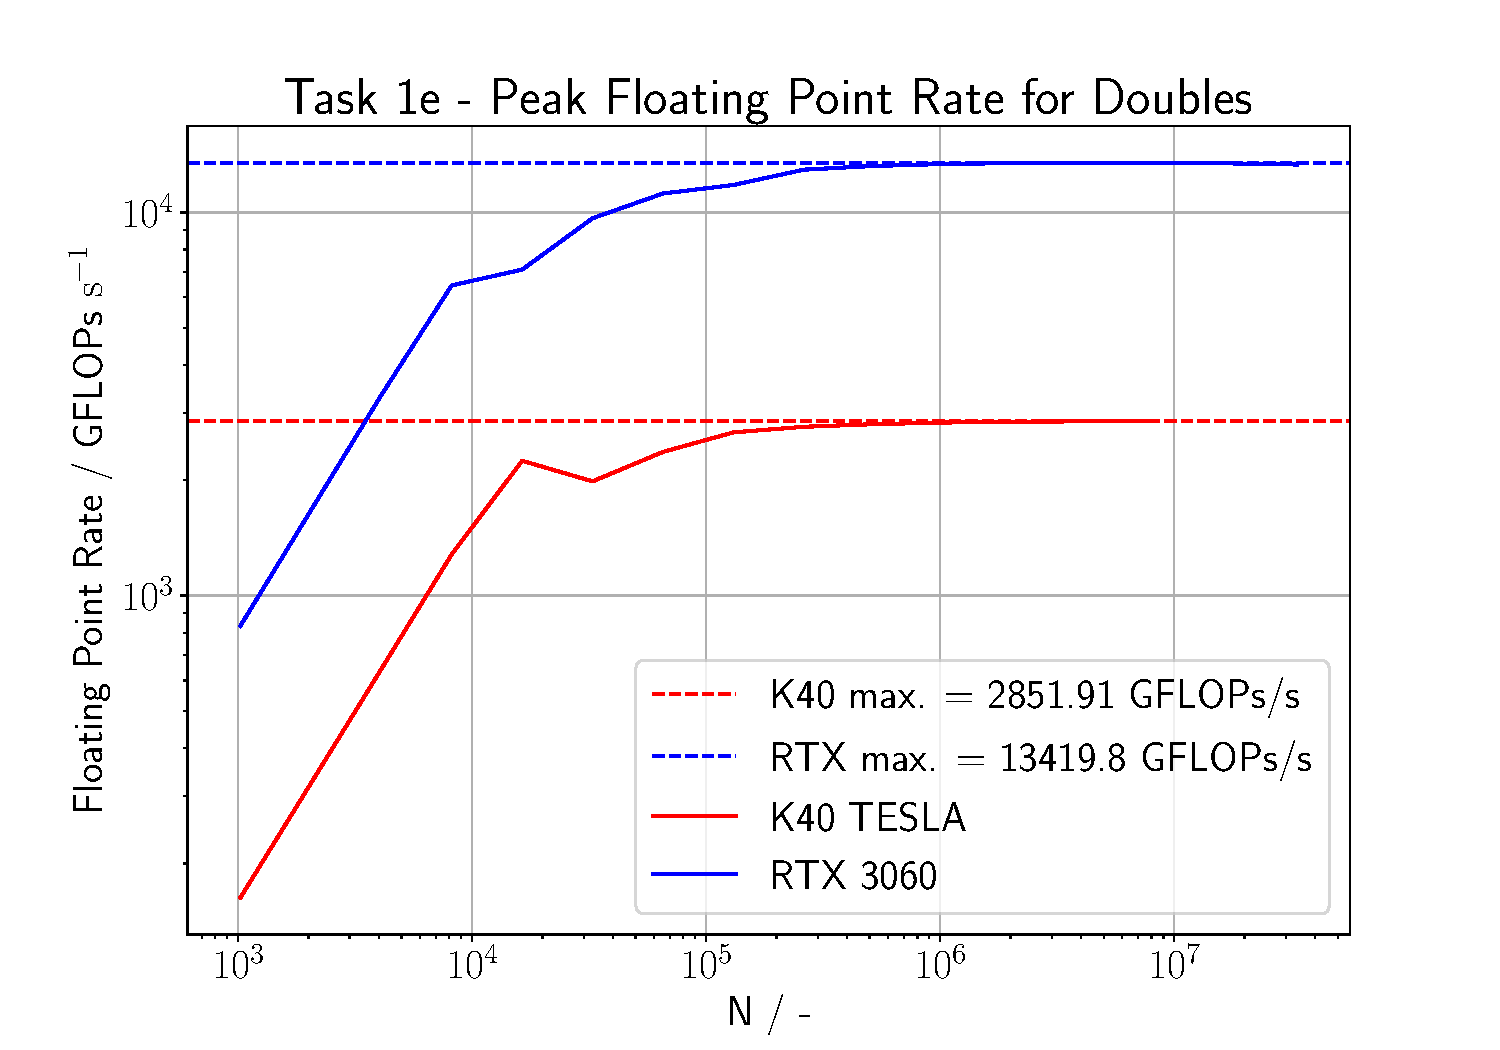
\includegraphics[width= 0.8\linewidth]{figures/task_1_e.pdf}
    \caption{}
    \label{label_1e_figure}
  \end{center}
\end{figure}

\pagebreak